\chapter{How to Speak So That People Want to Listen}

This lecture is compact, but its structure is unusually clean. It begins with a paradox: the human voice is enormously powerful, yet many of us know the experience of speaking without being heard. Treasure resolves that paradox in three stages. First he diagnoses the habits that make listening collapse. Then he proposes a positive foundation for speech. Only after that does he open the vocal toolbox itself, turn the toolbox into a warm-up routine, and finally widen the whole discussion into a picture of a better world of sound.

\section{The Voice and the Problem}

The lecture opens at full scale. The human voice, we are told, is the instrument we all play. It may be the most powerful sound in the world. It can start a war; it can say ``I love you.'' The point of this opening is not ornament. It is to force the problem into view. If the medium is so strong, why does it so often fail in practice?

Treasure asks the question directly: why is it that when many people speak, others do not listen? And how can we speak powerfully enough to make change in the world? This question governs the rest of the lecture. We may summarize its structure in a compact editorial way as follows:
\begin{equation}
\text{powerful medium} \;\not\Rightarrow\; \text{effective communication}.
\end{equation}
Something else has to intervene between the capacity of the voice and the willingness of others to attend to it.

\subsection{Question \& Answer}

\paragraph{Question.} Why do people fail to listen when we speak?

\paragraph{Answer.} Treasure's answer is layered. First, certain habits destroy listenability before technique even enters the picture. Second, even when our intentions are sound, delivery matters: the same words can arrive with very different force, clarity, and meaning depending on how they are spoken. The lecture therefore moves first through diagnosis, then through foundations, and only then through mechanics.

\section{The Seven Deadly Sins of Speaking}

Treasure's first answer is negative. He does not begin by telling us what to do; he begins by cataloguing what to stop doing. The seven ``deadly sins'' are not presented as exhaustive, but as large recurring habits that reliably make speech hard to hear.

In a compact notation, useful for the architecture of the notes though not written by the lecturer, we may collect them as
\begin{equation}
S_7 =
\bigl(
\text{gossip},
\text{judging},
\text{negativity},
\text{complaining},
\text{excuses},
\text{embroidery},
\text{dogmatism}
\bigr).
\end{equation}

\begin{remark}
This notation is editorial. Its purpose is to preserve the lecture's deliberate sequence and make the classification easy to carry forward.
\end{remark}

Each item does a specific kind of damage.

\paragraph{Gossip.} Speaking ill of someone who is not present poisons the speaking situation immediately. If a person gossips about others in front of us, we naturally infer that the same person will gossip about us later. Listening is already weakened by the loss of trust.

\paragraph{Judging.} It is difficult to listen to someone while feeling simultaneously judged and found wanting. The lecture's point here is relational rather than moralistic: a judging speaker makes the listener self-conscious, and self-consciousness interrupts attention.

\paragraph{Negativity.} Treasure gives this sin texture by example. His mother's late-life habit of saying, in effect, that even October 1 is dreadful is funny on the page because it is painful in life. Persistent negativity narrows the listener's world until speech becomes an instrument of contraction.

\paragraph{Complaining.} Treasure treats complaining as another form of negativity, but he lets it stand as its own recognizable habit. He calls it viral misery. It spreads discontent rather than light.

\paragraph{Excuses.} The figure here is the person with a blame-thrower, someone who passes responsibility on to everybody else. Again the lecture's emphasis is practical: such a speaker is hard to listen to because responsibility never lands anywhere stable.

\paragraph{Embroidery.} By embroidery he means exaggeration. Language is inflated until it loses calibration. If everything is awesome, then nothing is. And when exaggeration continues far enough, it turns into lying.

\paragraph{Dogmatism.} Dogmatism is the confusion of facts with opinions. Once those two are conflated, the listener is no longer being invited into inquiry but bombarded by assertion masquerading as truth.

The movement of the section is cumulative. Treasure is not saying merely that these habits are bad. He is showing that each one breaks the channel between speaker and listener in a distinct way. By the end of the list, we have a rigorous negative answer to the opening problem: often people do not listen because we have made ourselves difficult to listen to.

\section{HAIL: The Positive Foundations}

Having diagnosed the failures, Treasure pivots sharply: is there a positive way to think about this? The answer is yes, and it comes in the form of a second compressed structure. The four foundations spell the word HAIL. In compact notation:
\begin{align}
H &\mapsto \text{honesty},\\
A &\mapsto \text{authenticity},\\
I &\mapsto \text{integrity},\\
L &\mapsto \text{love}.
\end{align}

Treasure likes the word not only because it is memorable, but because it also means to greet or acclaim enthusiastically. If we stand on these four things, the suggestion is that our words may be received that way.

\begin{figure}[h]
\centering
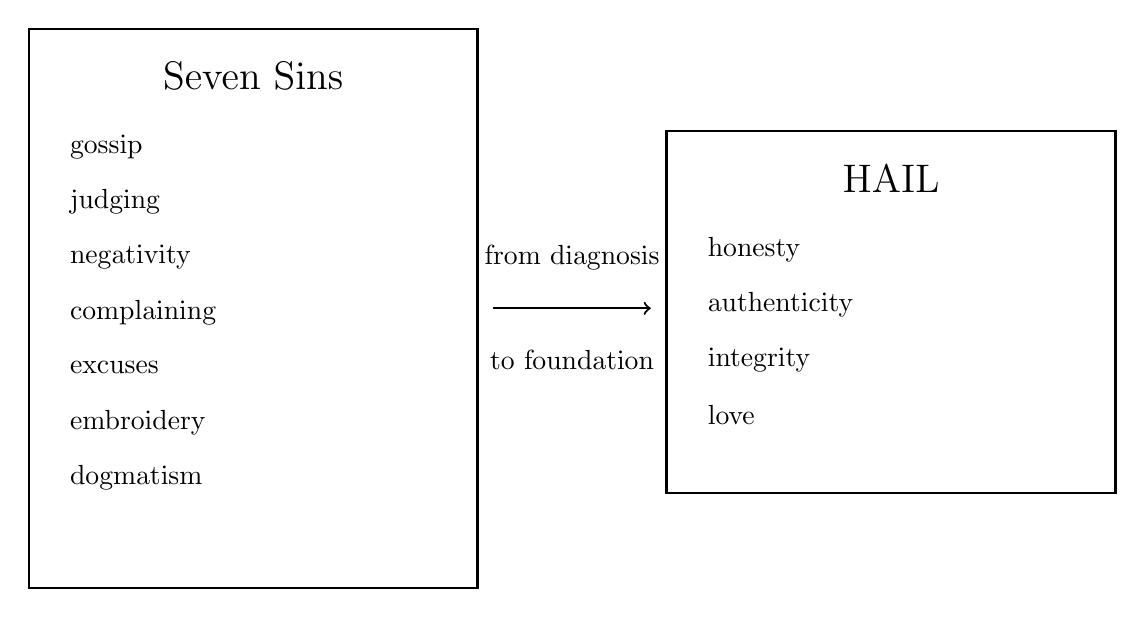
\begin{tikzpicture}[x=1cm,y=1cm]
\draw[thick] (0,0) rectangle (5.7,7.1);
\draw[thick] (8.1,1.2) rectangle (13.8,5.8);
\node at (2.85,6.5) {\Large Seven Sins};
\node at (10.95,5.2) {\Large HAIL};

\node[anchor=west] at (0.4,5.6) {gossip};
\node[anchor=west] at (0.4,4.9) {judging};
\node[anchor=west] at (0.4,4.2) {negativity};
\node[anchor=west] at (0.4,3.5) {complaining};
\node[anchor=west] at (0.4,2.8) {excuses};
\node[anchor=west] at (0.4,2.1) {embroidery};
\node[anchor=west] at (0.4,1.4) {dogmatism};

\node[anchor=west] at (8.5,4.3) {honesty};
\node[anchor=west] at (8.5,3.6) {authenticity};
\node[anchor=west] at (8.5,2.9) {integrity};
\node[anchor=west] at (8.5,2.2) {love};

\draw[->,thick] (5.9,3.55) -- (7.9,3.55);
\node at (6.9,4.2) {from diagnosis};
\node at (6.9,2.9) {to foundation};
\end{tikzpicture}
\end{figure}

The schematic above is not extracted from a validated frame. It is a transcript-derived map of the lecture's first major transition: from habits to be abandoned to principles on which speech can stand.

\subsection{Question \& Answer}

\paragraph{Question.} What positive foundation replaces the seven sins?

\paragraph{Answer.} Treasure's answer is that powerful speech must be truthful, real, dependable, and benevolent. Honesty keeps language straight. Authenticity prevents us from speaking through a mask. Integrity makes us somebody others can trust. Love ensures that speech is directed toward the good of the listener rather than toward domination or vanity.

The most interesting local tension appears in the letter \(L\). Treasure does not say merely that love is nice. He uses it to qualify honesty. In a compact symbolic form we may summarize his point as
\begin{equation}
\text{absolute honesty} \not\Rightarrow \text{good speech},
\qquad
\text{honesty tempered with love} \Rightarrow \text{good speech}.
\end{equation}
His example is memorable because it is so plain: ``You look ugly this morning'' may be honest, but it is not therefore necessary. Love does not cancel honesty; it constrains its use.

He adds a second observation:
\begin{equation}
\text{love} \;\Rightarrow\; \text{difficulty in judging at the same time}.
\end{equation}
This is not a theorem. It is a qualitative incompatibility. If we are genuinely wishing somebody well, the judging stance becomes much harder to maintain. In this way the letter \(L\) also answers one of the original sins.

\section{The Vocal Toolbox}

Treasure now makes his next major pivot. It is not only what we say; it is the way that we say it. The voice becomes, in his language, an amazing toolbox that very few people have ever opened. This is the technical center of the lecture.

For purposes of note-taking, we may gather the variables into a single ordered object:
\begin{equation}
V_{\text{tool}}=
\bigl(
\text{register},
\text{timbre},
\text{prosody},
\text{pace},
\text{silence},
\text{pitch},
\text{volume}
\bigr).
\end{equation}

\paragraph{Register.} Treasure contrasts the voice placed ``in the nose,'' ``in the throat,'' and ``in the chest.'' He is not offering acoustic physiology in detail; he is offering a practical phenomenology of placement. The argument is that if we want weight, we tend to go lower, toward the chest. He adds the memorable rhetorical claim that we vote for politicians with lower voices because we associate depth with power and authority. In shorthand:
\begin{equation}
\text{lower register} \;\Rightarrow\; \text{greater perceived power and authority}.
\end{equation}

\paragraph{Timbre.} Timbre is the felt texture of the voice. Treasure says that the research prefers voices that are rich, smooth, and warm, like hot chocolate. The important point for the notes is not the metaphor alone, but the trainability claim: timbre can be improved through breathing, posture, and exercise. The voice is not fixed at its current state.

\paragraph{Prosody.} Prosody, the sing-song meta-language of speech, is one of Treasure's most important technical ideas. He calls it route one for meaning in conversation. This is why monotone delivery is so hard to hear: it suppresses a primary carrier of meaning.

\subsection{Question \& Answer}

\paragraph{Question.} Why can the same words mean different things when delivered differently?

\paragraph{Answer.} Because meaning is not a function of words alone. Treasure's demonstrations with repetitive question-ending intonation and with the sentence ``Where did you leave my keys?'' show that prosody and pitch change the force of an utterance even when the lexical content is held fixed.

In a compact editorial notation, let
\begin{align}
u &= \text{``Where did you leave my keys''},\\
m_1 &= \mathcal{M}(u,\pi_1),\\
m_2 &= \mathcal{M}(u,\pi_2).
\end{align}
Here \(\pi_1\) and \(\pi_2\) denote different prosodic or pitch contours, and \(\mathcal{M}\) is the meaning assigned by a listener. Treasure's point is simply that
\begin{equation}
m_1 \neq m_2.
\end{equation}
The lexical string has not changed. The contour has changed, and so the speech act has changed with it.

This is the context for his complaint about repetitive question-ending prosody. When every sentence rises as if it were a question, statements lose their declarative force. A speaker who uses only one contour has restricted the expressive space.

\paragraph{Pace and silence.} Treasure demonstrates pace by contrast. One can accelerate to generate excitement, or slow down to create emphasis. And at the far edge of pacing lies silence. Silence is not dead air to be filled with ``ums'' and ``ahs''; it is a communicative resource. In the lecture's logic,
\begin{equation}
\text{fast pace} \Rightarrow \text{excitement},
\qquad
\text{slow pace} \Rightarrow \text{emphasis},
\qquad
\text{silence} \Rightarrow \text{powerful punctuation}.
\end{equation}

\paragraph{Pitch.} Pitch often works together with pace, but Treasure shows that it can also act on its own. The two deliveries of the same sentence differ because the melodic contour differs. Again, the argument is not acoustical in the narrow sense; it is semantic. The listener hears different intent.

\paragraph{Volume.} Volume is the last tool in the block. Loudness can generate command and excitement. Quietness can pull a room inward and make people pay attention. Treasure's warning is against constant broadcasting, which he names ``sodcasting'': the inconsiderate imposition of sound on everyone nearby.

The deep point of the whole section is that speech can be shaped as a controlled multi-variable system. Treasure is not merely telling us to ``sound better.'' He is enumerating parameters that we can vary, and then demonstrating what those variations do.

\section{Preparing the Instrument}

Once the toolbox has been opened, Treasure moves from analysis to preparation. The transition is entirely motivated: when something really matters, whether a public talk, a proposal, a request for a raise, or a wedding speech, we owe it to ourselves to prepare the instrument. He then introduces the engine metaphor: no engine works well without being warmed up.

\subsection{Question \& Answer}

\paragraph{Question.} Why warm up the voice before speaking?

\paragraph{Answer.} Because the voice is not merely a message channel; it is an instrument with moving parts. If important speech deserves preparation, then the instrument that will carry that speech deserves preparation too. Treasure therefore turns the talk into a live protocol.

We may compress the protocol as
\begin{equation}
W_6=
\bigl(
\text{breath},
\text{lips},
\text{trill},
\text{tongue},
\text{rolled } r,
\text{siren}
\bigr),
\end{equation}
but the real value lies in the ordered steps:

\begin{enumerate}
\item Raise the arms, take a deep breath, and sigh out.
\item Warm up the lips with repeated ``bop'' sounds.
\item Continue with the lip trill, like a child making a motor sound.
\item Wake up the tongue with exaggerated ``la, la, la'' articulation.
\item Roll an \(r\), which Treasure calls ``champagne for the tongue.''
\item Finish with the siren: move from high ``we'' down to low ``or.''
\end{enumerate}

The sequence is pedagogically important. It turns the lecture's abstract account of register, timbre, and articulation into a pre-performance routine. Treasure does not leave the toolbox as theory; he makes the audience use it.

\section{Closing Vision: The World of Conscious Sound}

The lecture closes by widening its scope. Treasure says explicitly that he wants to put the discussion in context. The present world, as he describes it, is one in which we often speak poorly to people who are not really listening, in environments dominated by noise and bad acoustics. In a compact synthesis,
\begin{equation}
\text{current world}
=
\bigl(
\text{poor speaking},
\text{poor listening},
\text{noise},
\text{bad acoustics}
\bigr).
\end{equation}

The counterfactual world he imagines is one in which speech is powerful, listening is conscious, and environments are designed with sound in mind:
\begin{equation}
\text{desired world}
=
\bigl(
\text{powerful speaking},
\text{conscious listening},
\text{conscious sound creation},
\text{fit-for-purpose acoustics}
\bigr).
\end{equation}

This is an important broadening. The lecture does not end with the individual speaker alone. It ends with a social acoustics. The question is no longer only how we as individuals can speak better. It becomes what sort of world we would inhabit if speaking, listening, and acoustic design were all undertaken consciously.

The final payoff is therefore not merely eloquence. It is understanding. A world that sounds beautiful, Treasure says, would also be a world in which understanding is the norm. The ending gives the talk its last lift: a lecture that began with the power of the voice ends by asking what sort of human world that power might build if we finally learned to use it.

\section{Summary}

Treasure's lecture is built from nested ordered structures. We begin with a paradox: the voice is powerful, yet people do not listen. We answer negatively with the seven sins, positively with HAIL, technically with the vocal toolbox, practically with the six warm-ups, and finally socially with a vision of conscious sound.

What makes the lecture effective is that each new structure is motivated by the previous one. The sins explain why the channel fails. HAIL rebuilds trust. The toolbox shows how delivery shapes meaning. The warm-ups turn knowledge into practice. And the ending widens personal craft into a world-model. If we keep that order on the page, the notes will preserve the lecture's real argument: not merely that speaking matters, but that powerful speech is a disciplined combination of ethical stance, vocal control, preparation, and attention to the world in which sound is made.